\chapter{Manual Annotation} \label{chapter:manual_annotation}

\begin{figure}[!tbp]
	\centering
    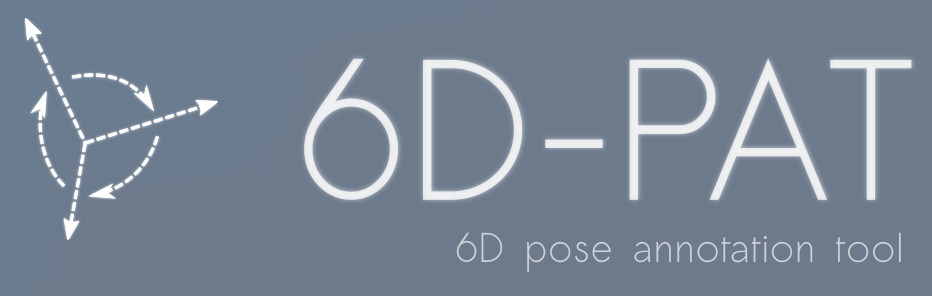
\includegraphics[width=0.8\linewidth]{6dpat}
    \caption{The logo of the pose annotation tool \ac{6dpat}.}
    	\label{fig:6dpat_logo}
\end{figure} 

The following chapter analyzes the manual 6D pose annotation process and its prerequisites. To this end, we define the necessary terminology and explain the workflow of recovering poses from images using the tool we developed. 

\section{Terminology} \label{section:terminology}

\textbf{Image.} An image $I$ is a 2D matrix of pixels. The pixel $u$ at position $(i, j)$ is referenced by the tuple $(x, y)$, where $x = j$ and $y = i$. The author of this work chose this notation over the row-major matrix indexing because images are often column-major indexed. \\

\noindent\textbf{Object Model.} An \textit{object model} (or \textit{3D model}) $O$ is composed of a set of points $M \subseteq \mathbb{R}^3$ and a set of triangles $T \subseteq M^3$, also called a mesh. The type of object is not restricted. In the T-Less dataset \cite{tless}, the objects are mostly screws and other hardware. \\

\noindent\textbf{6D Pose.} A \textit{6D pose} $P$ is the tuple $(R, t)$. $R$ is the $3\times 3$ rotation matrix and $t \in \mathbb{R}^3$ the translation vector used to transform an object model into camera coordinates (see Section \ref{objectcoordinates}). \\

\noindent\textbf{Correspondence.} A \textit{correspondence} $C$ is the tuple $(u, p)$, which captures the relation between a pixel $u$ of an image $I$ and a 3D point $p$ on the surface of an object model $O$. The pixel $u$ is the projection of $p$ onto the image plane using the camera matrix $K$ and a pose $P$. A pose can be recovered computationally if at least three correspondences are known (see Section \ref{objectcoordinates}). \\

\noindent\textbf{Segmentation Mask.} A \textit{segmentation mask} (or \textit{segmentation image}) $S$ for an image $I$ is a second image of the same size. Each position $(x, y)$ of the mask encodes the class of the pixel at $(x, y)$ in $I$. The set of classes can be defined arbitrarily. In the context of this work, each class represents a type of object model. The segmentation mask can be seen as the mapping $s(x, y) = q_i$ for a class set $Q = \{q_0, \cdots, q_n\}$. \\

\noindent\textbf{Ground-Truth.} A \textit{ground-truth pose} $\bar{P}$ is a 6D pose, which is always recovered by a human instead of a machine. The ground-truth pose is the best approximation of the rotation and translation of an object model $O$ visible in an image $I$. It is an approximation because there can be a discrepancy between the real world object and its digital 3D representation. Image conditions like lightning, motion blur, etc. might make it unfeasible to recover the perfect pose. Camera distortions and other influences in the photographs of the objects might also not be modeled correctly or not accounted for at all. But it must apply that the translation and rotation error of a ground-truth pose $\bar{P}$ are within a certain threshold. \\

\noindent\textbf{Depth Image.} A \textit{depth image} is an image $D$ belonging to an image $I$ of the same size that contains the distance $d$ between the camera and the surface for each pixel $u$ in $I$. Depth images can be obtained from stereo images or using special cameras and are often used in pose estimation and other computer vision tasks. A depth image can also be denoted by \textit{RGB-D}.

\begin{figure}[!tbp]
	\centering
	\begin{subfigure}[t]{0.47\textwidth}
	\centering
    	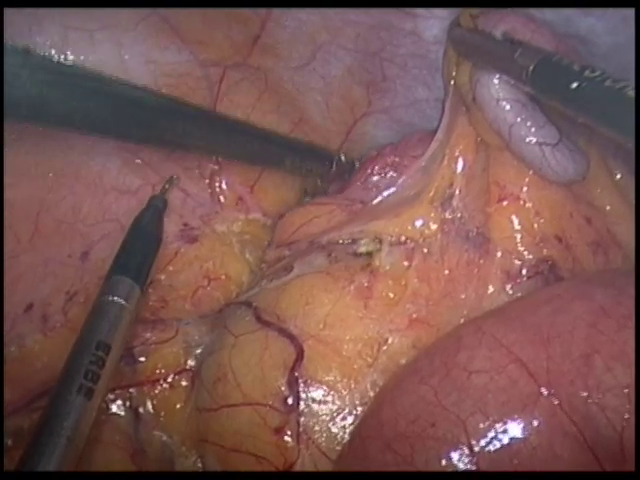
\includegraphics[width=0.8\linewidth]{sfb_original}
    	\caption{An example image from the Endoscopic Vision Challenge dataset. Image from \cite{endovis}.}
    	\label{fig:sfb_original}
	\end{subfigure}
	\hfill
	\begin{subfigure}[t]{0.47\textwidth}
	\centering
    	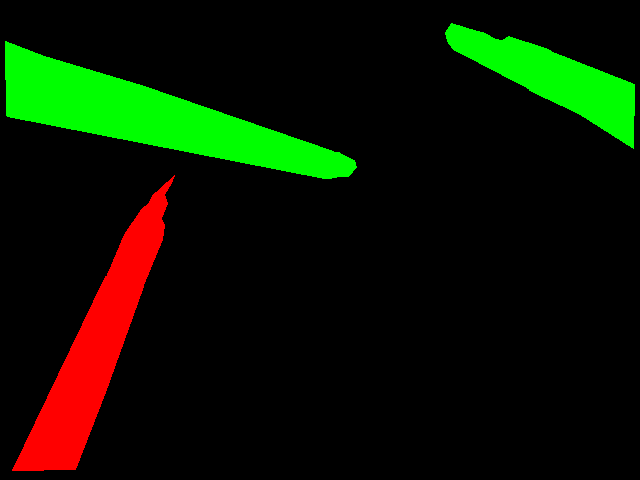
\includegraphics[width=0.8\linewidth]{sfb_segmentation}
    	\caption{The corresponding segmentation mask. The colors encode the tools' classes. Image from \cite{endovis}.}
    	\label{fig:sfb_segmentation}
	\end{subfigure}
	\caption{An example image and its corresponding segmentation mask from the Endoscopic Vision Challenge dataset.}
	\label{fig:sfb}
\end{figure} 

\section{Images of the Endoscopic Vision Challenge}

The goal of this work is to provide a system to successfully and efficiently annotate the images of the \textit{Endoscopic Vision Challenge} \cite{endovis}. The dataset includes segmentation masks but neither object models nor pose annotations or depth images. An example image together with the corresponding segmentation mask are given in \fig \ref{fig:sfb}. Occlusion and artifacts like motion blur can occur in the images. The issues with this dataset and the obstacles preventing its complete annotation are discussed Section \ref{section:6dpat_difficulties}. 

\section{6D Pose Annotation Tool (6D-PAT)}

The creation of sufficient training data for neural networks can be a time-consuming and tedious process. Using non-specialized tools designed for other purposes, like 3D modeling or CAD programs, require the person creating the annotations to get accustomed to complex user interfaces (\acp{ui}). The goal of the annotation tool is to provide a system that allows easy and efficient annotation of images - images of the Endoscopic Vision Challenge in particular. The ground-truth poses recovered using the program can then be used to train a neural network. The program is written mainly in the language C++ and is dubbed \textit{\acf{6dpat}}. Its logo can be seen in \fig \ref{fig:6dpat_logo}. The next sections present the carved out requirements, details on the used frameworks, the program's architecture, as well as the designed pose recovery process.

\subsection{Requirements}

Fulfilling the goal of providing a tool for annotating large datasets implies some requirements. Datasets can consist of thousands of images and many object models. To guarantee a fluid workflow, we need to provide the user with a browsable overview over the dataset. This prevents a disruptive annotation process, as the user doesn't need to open the next image or a different object model individually after recovering a pose. The program has to offer the possibility to select and view images and object models, respectively. The most essential part of such an annotation tool is the incorporation of functionality to recover poses and to edit misaligned poses. Different manual pose recovery mechanisms are possible. Due to the limited time frame of this work, we implemented only one method, which we expected to be the most efficient one. The annotation process is described in detail in Section \ref{subsection:correspondence_and_pose_creation}.

\subsection{Frameworks \& Third-Party Libraries}

All necessary dependencies of the tool are listed below. The user needs to compile or install the dependencies before using the annotation tool. But since all frameworks and libraries are platform-independent, the program can be compiled and run on different systems. \\

\noindent\textbf{Qt.} \textit{Qt} \cite{qt} is a powerful framework for C++ that offers a vast selection of user interface components but also general functionality that exceeds the capabilities of the standard C++ library. Qt was also chosen as the main framework because it ensures portability of C++ applications by encapsulating system calls of all kind. \\

\begin{figure}[!tbp]
	\centering
	\begin{subfigure}[t]{0.47\textwidth}
		\centering
    	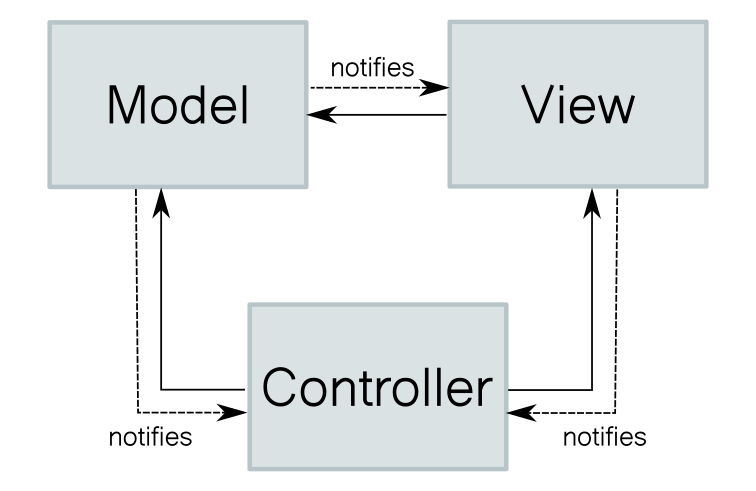
\includegraphics[width=0.8\linewidth]{mvc}
    	\caption{The Model-View-Controller architecture. The solid lines stand for a direct connection either because the target is owned or known by reference. The dashed line is an indirect connection realized using the observer pattern or the Qt Signals and Slots mechanism.}
    	\label{fig:mvc}
	\end{subfigure}
	\hfill
	\begin{subfigure}[t]{0.47\textwidth}
	\centering
    	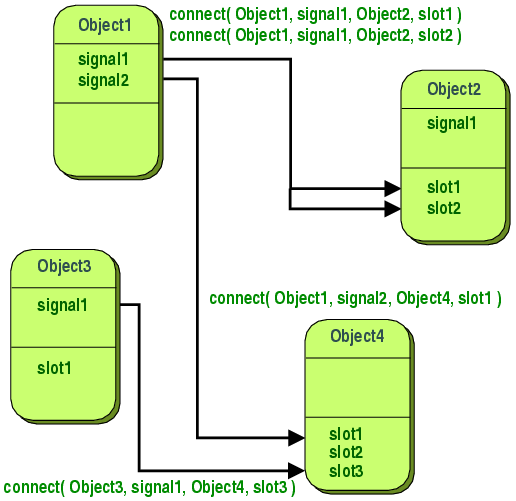
\includegraphics[width=0.8\linewidth]{qt_signals_slots}
    	\caption{The Signals and Slots mechanism of Qt. A class can define signals which can be emitted. Slots are functions that can be connected to signals. When a signal is emitted, all connected slots will be called. Image from \cite{qt_signals_and_slots}.}
    	\label{fig:qt_signals_slots}
	\end{subfigure}
	\caption{Two basic architectural concepts used in \ac{6dpat}: the model view controller pattern and the signal and slots pattern.}
\end{figure} 

\noindent\textbf{OpenGL.} \textit{OpenGL} \cite{opengl} is a widespread open-source 3D graphics library specification. Implementations of the specification exist for many different operating systems, which makes applications using OpenGL portable. \\

\noindent\textbf{OpenCV.} \textit{OpenCV} \cite{opencv} is a C++ library created for various computer vision tasks. OpenCV provides functions for object tracking, object detection, image segmentation and many more. We use its \textit{solvePnPRansac} method in this work. \\ 

\noindent\textbf{Assimp.} \textit{Assimp} \cite{assimp} is a C++ library designed to import 3D models. The library was incorporated into the tool to ensure a broad support of 3D model formats.

\subsection{Architecture \& Code Design}

\ac{6dpat} is primarily a \ac{ui} program, i.e. its purpose is to display a window and enable optical interaction for the user. Thus, we chose the \textit{\ac{mvc}} pattern as the underlying architecture. \ac{mvc} separates the concerns of data management (Model), displaying data (View) and high level logic (Controller). The schematic of the \ac{mvc} architecture is shown in \fig \ref{fig:mvc}. To ensure extensibility and exchangeability, the classes of the model do not know view or controller classes directly. The model only informs its observers (views that display data, for example) through indirect connections. The indirect connections are realized via Qt's signals and slots mechanism, which is visualized in \fig \ref{fig:qt_signals_slots}. The view classes only display data and handle simple user interactions that do not involve complex logic. The latter is the responsibility of the controller classes. Classes do not know implementation details of classes of other groups. To speed up interface creation, we used \textit{Qt Designer} to layout the views. Qt Designer is a graphical tool that allows placement of \ac{ui} components and linking of signals and slots without directly writing code and is part of the standard Qt framework.

\begin{figure}[!tbp]
       \centering
   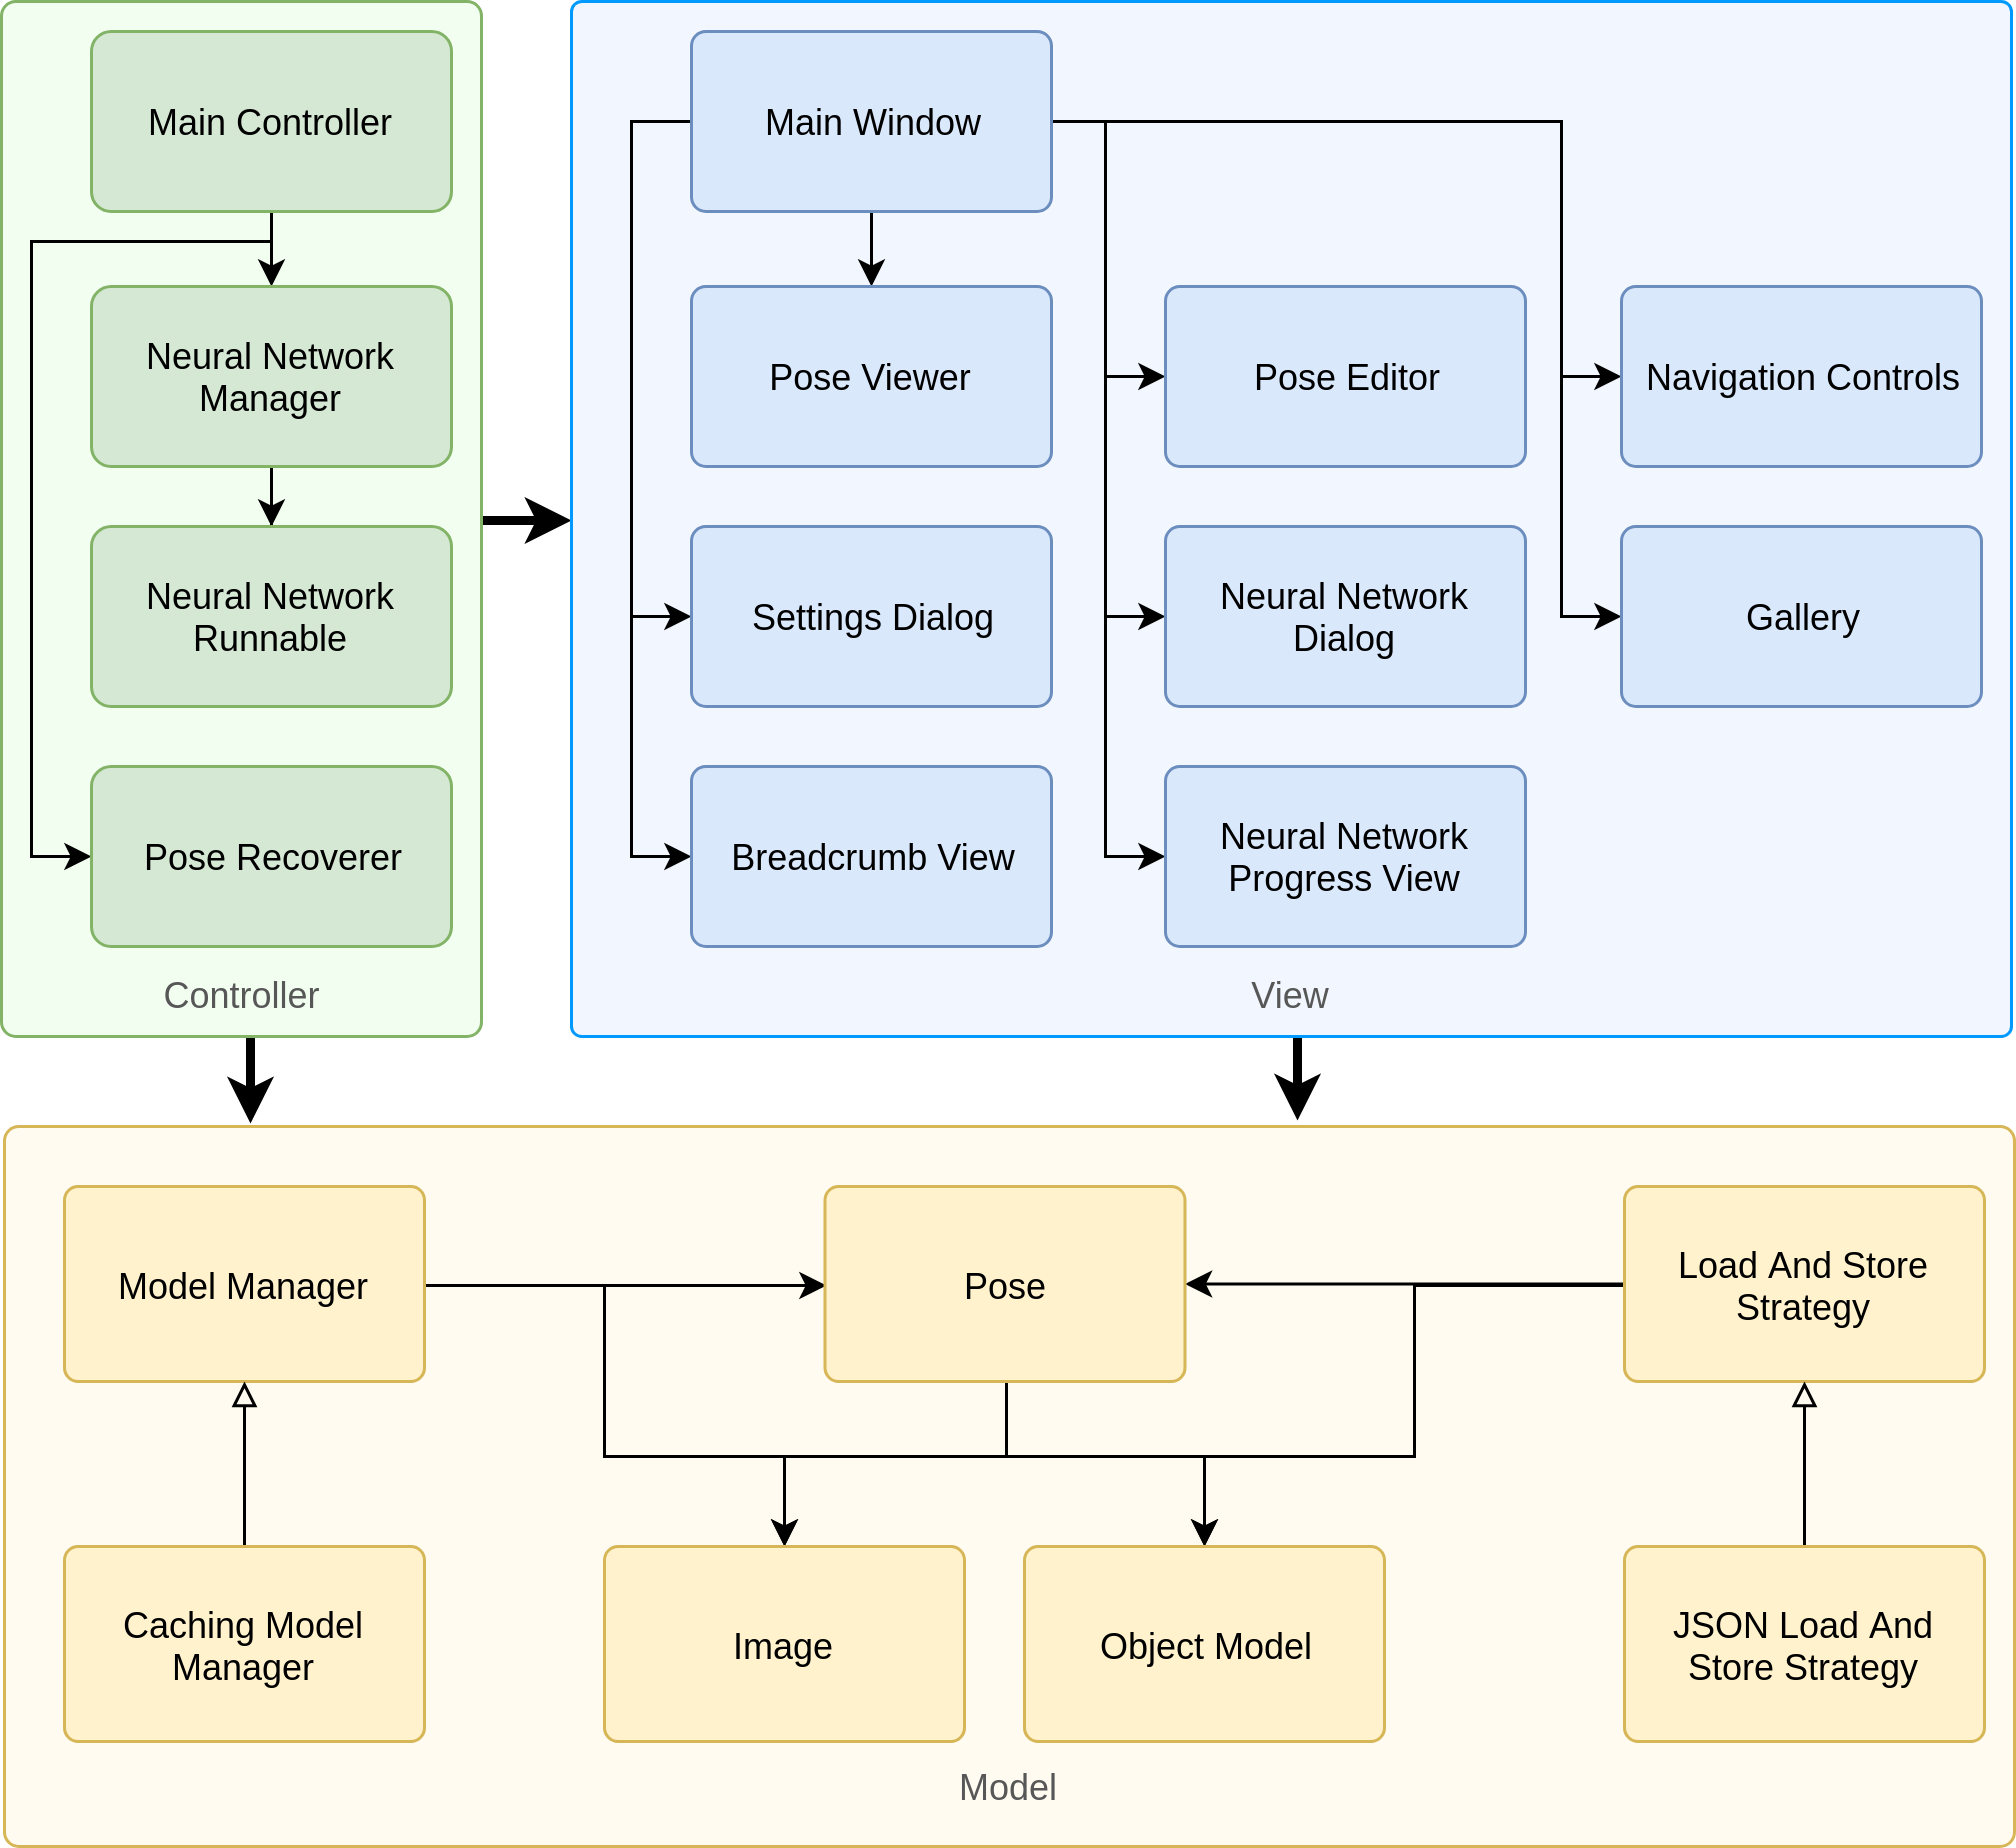
\includegraphics[width=\linewidth]{6dpat_class_diagram}
    \caption{An abstract high-level class diagram of a subset of the classes of \ac{6dpat}. The large rectangles show the affiliation of a contained class in the \ac{mvc} pattern. Arrows between those rectangles imply which class can use which target class, although not all classes of the source rectangle necessarily use all classes of the target rectangle. Small filled-out arrows imply a use relationship, while the not filled-out arrow heads indicate inheritance.}
   \label{fig:6dpat_class_diagram}
\end{figure}

The most important classes of the program are displayed in \fig \ref{fig:6dpat_class_diagram}. The diagram is simplified for easier understanding. The large rectangles group the classes by their affiliation in the \ac{mvc} pattern. The bold arrows between the groups denote which classes can use or know which other classes. This does not necessarily mean, that all classes of the source rectangle use all classes of the target rectangle. 

\subsubsection{Controller Classes}

The controller classes consist mostly of the \textit{Main Controller}, which owns the \textit{Pose Recoverer} and the \textit{Neural Network Manager}. The code of these classes has not been incorporated into the main controller to further separate the classes by concern and facilitate future modifications. The pose recoverer handles the clicked 2D-3D correspondences and offers functionality to compute the pose. The neural network manager handles all tasks of the network. To keep the \ac{ui} responsive during time-consuming network operations, the network manager uses the \textit{Neural Network Runnable} to run tasks in a separate thread. This design allows easy substitution of how to the network is run, if necessary. The main controller also creates the \textit{Model Manager} and the \textit{Load And Store Strategy}. To use different implementations of either class, the controller has to be adjusted to create those instead. The \textit{Main Window} is created by the main controller, as well, and receives the model manager from it.

\subsubsection{View Classes}

The main window holds all views of the \ac{ui}. It is the central partner for the main controller on the view side and delegates all alterations requested by the controller to the other views. All signal and slots that are necessary between view classes get connected by the main window, if not defined in the Qt Designer. Most of the signals and slots communication takes place between the \textit{Pose Viewer}, the \textit{Pose Editor} and the galleries. Whenever the user clicks an image or an object model in the gallery, the gallery notifies the viewer and editor to display the respective entity. The view classes know the model classes, especially the model manager, by reference. They receive the reference from the main window. The pose viewer and editor communicate to show the alterations made to a pose before saving the changes. Simple operations, like saving an edited pose, are often directly processed by the view classes to reduce the amount of signals and slots.

\subsubsection{Model Classes}

The model manager and the load and store strategy are the key interfaces to access data. The actual code of managing the data was separated into the \textit{Caching Model Manager}, which caches the list of images, object models and poses, and the \textit{JSON Load And Store Strategy}, which uses JSON files to store the poses. It expects the camera matrices file of the images to be in JSON format, as well. Both classes can be replaced to support database functionality in the future, for example. The classes that contain the actual data are the \textit{Image}, the \textit{Object Model} and the \textit{Pose} class. Class image references the path to an image and stores the corresponding camera matrix. Class object model stores the path to an object model. This allows loading the entities when need. The pose class holds a reference to the participating image and object model, as well as the respective rotation matrix and translation vector. 

\subsubsection{Miscellaneous Classes}

Some classes are not displayed in \fig \ref{fig:6dpat_class_diagram}, as they were deemed not important to understand the architecture of the program.

\subsection{Manual Annotation} 

This section describes the user interface of \ac{6dpat} and the steps required to annotate images with 6D poses in detail. 

\subsubsection{Preparation}

\begin{figure}[!tbp]
	\centering
	\begin{subfigure}[t]{\textwidth}
		\centering
    	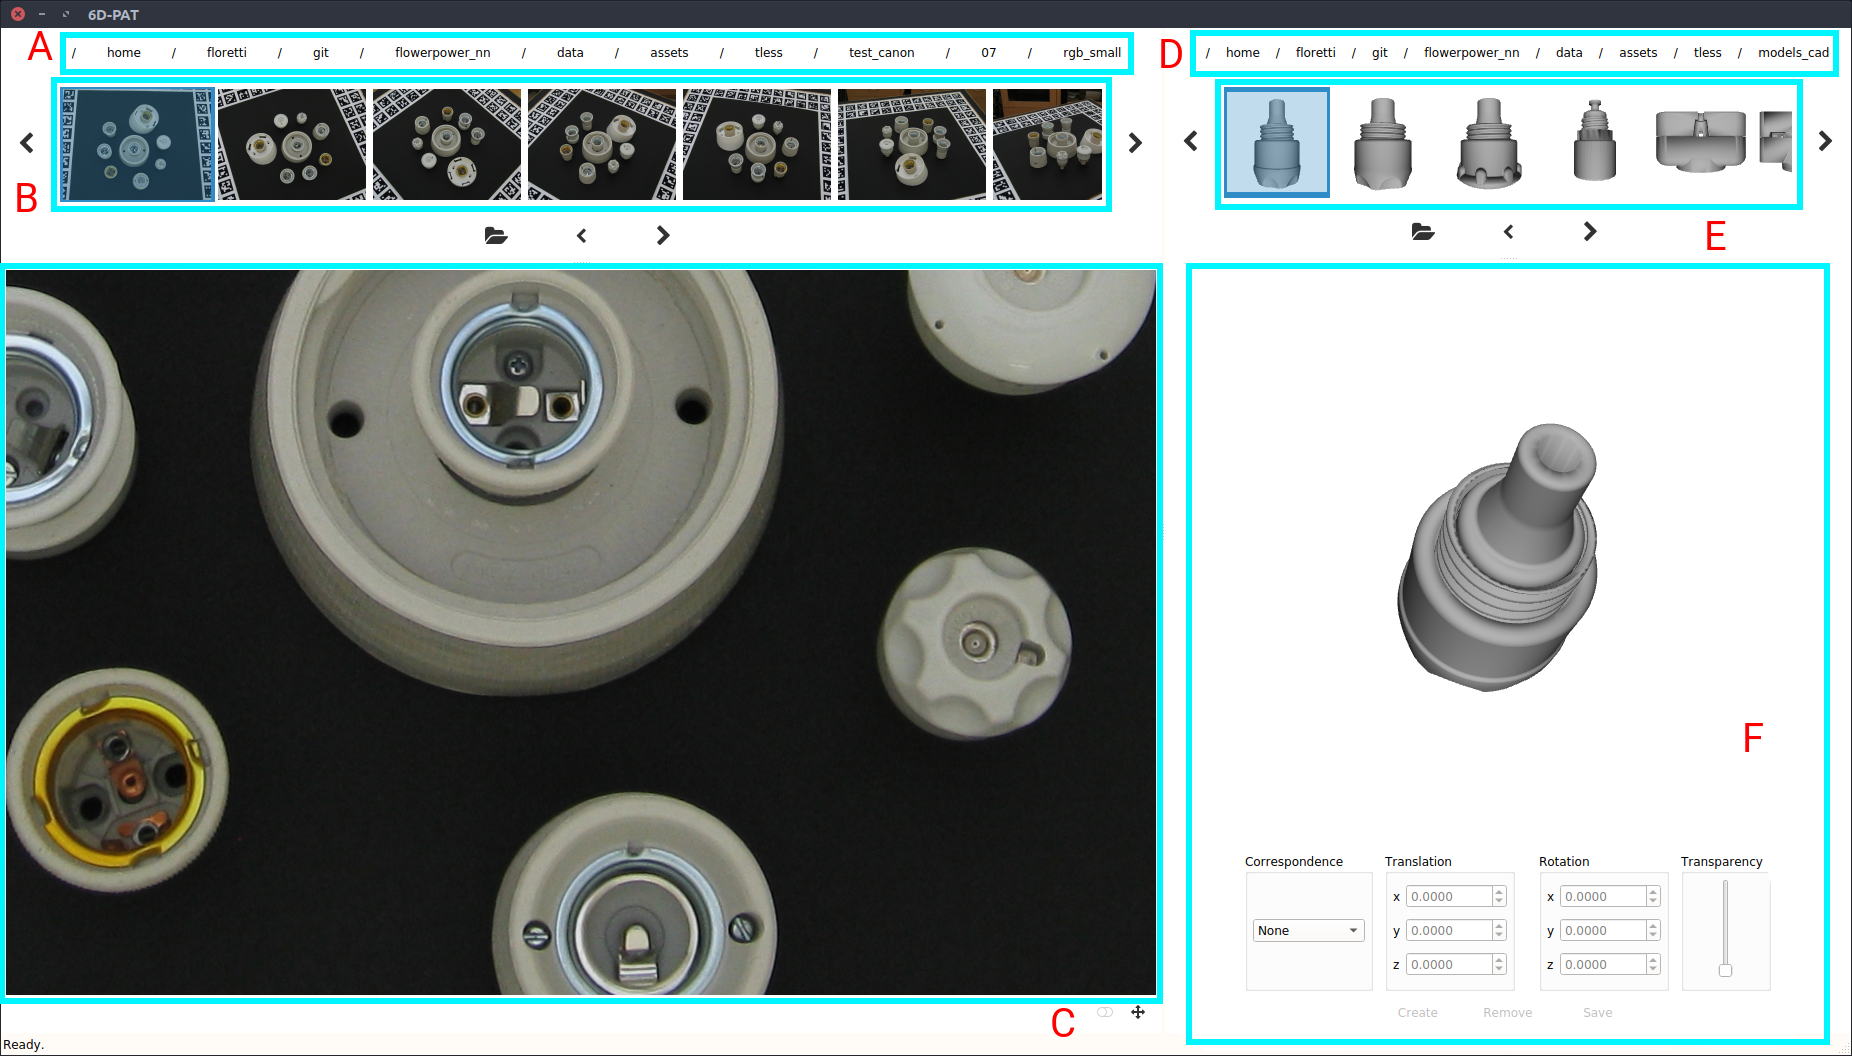
\includegraphics[width=\linewidth]{6dpat_components}
    	\caption{The user interface of the annotation tool \ac{6dpat}. The displayed images and object models are from the T-Less dataset. The following components are marked with a turquoise box: \textbf{A}: The full path of the currently selected folder to load images from. \textbf{B}: The \textit{Images Gallery} showing the images loaded from the selected path. \textbf{C}: The \textit{Pose Viewer} shows the image selected in gallery B. The user can click on the image to define the 2D starting point of a correspondence. \textbf{D}: The full path of the currently selected folder to load object models from. \textbf{E}: The \textit{Objects Gallery} of rendered 3D previews of the object models loaded from the selected path. \textbf{F}: The \textit{Pose Editor} shows the object model selected in gallery E. The user can click on the object model to complete the correspondence with the 3D point. The controls at the bottom can be used to edit existing poses.}
    	\label{fig:6dpat_components}
	\end{subfigure}
	\par\bigskip
	\begin{subfigure}[t]{0.47\textwidth}
		\centering
    	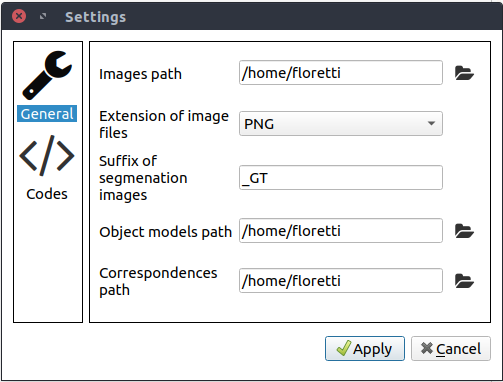
\includegraphics[width=\linewidth]{6dpat_settings}
    	\caption{The settings dialog of \ac{6dpat}. The dialog allows editing of the paths where the program loads images, object models and poses from.}
    	\label{fig:6dpat_settings}
	\end{subfigure}
	\hfill
	\begin{subfigure}[t]{0.47\textwidth}
	\centering
    	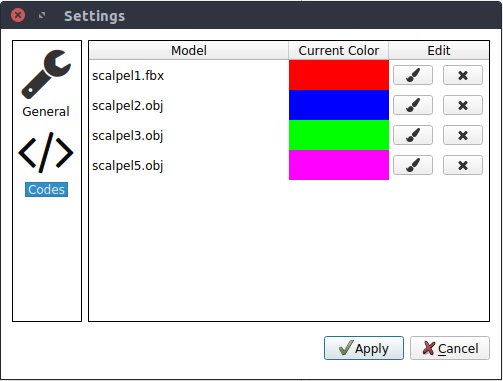
\includegraphics[width=\linewidth]{6dpat_settings_codes}
    	\caption{The tab of the settings dialog that can be used to assign colors to the object models.}
    	\label{fig:6dpat_settings_codes}
	\end{subfigure}
	\caption{The \ac{ui} of \ac{6dpat}.}
	\label{fig:6dpat_ui_overview}
\end{figure}

The first step after starting the program is to open the settings (see \fig \ref{fig:6dpat_settings}) and to set the path to the images that are to be annotated, as well as the path to the folder that contains the object models that are visible in the images. 

The folder of the images has to contain a JSON file that holds the camera matrix $K$ for each individual image. If no camera info file exists, a Python script that is distributed with the neural network can be used to create approximate camera matrices. The path to the segmentation images, if any, has to be set as well. The program loads the images and the segmentation images and sorts them by the numbers in their filenames and matches image $I$ at index $j$ with the segmentation image $S$ at index $j$. 

If segmentation images are present, they are linked to the respective image and can be viewed by activating the toggle at the bottom right corner of the pose viewer. The program displaying a segmentation image can be seen in \fig \ref{fig:sfb_segmentation}. 

Lastly, the user needs to specify the location of the JSON file where the program is supposed to load existing ground-truth poses from and write new ones to. If no such file exists, an empty one can be created and selected. 

If required, the user can assign colors to the object models using the settings dialog depicted in \fig \ref{fig:6dpat_settings_codes}. The colors should correspond to the color used in the segmentation mask. The object models gallery will automatically display only the object models whose color is present in the segmentation image of the currently viewed image. If no segmentation images exist, the gallery shows all object models.

\subsubsection{Creation of Correspondences and Pose Recovery} \label{subsection:correspondence_and_pose_creation}

\begin{table}
\centering
    \begin{tabular}{|c||ccccc|} \hline
\diagbox{\# Object}{Image} & 0000.jpg & 0150.jpg & 0250.jpg & 0350.jpg & 0500.jpg \\ \hline\hline
\rowcolor{Gray}
01           &  \textbf{2:09} (0:47) & \textbf{4:17} (1:05) & \textbf{1:31} (0:52) & \textbf{1:24} (0:55) & \textbf{1:15} (0:52) \\ 
        15 & \textbf{2:31} (0:56) & \textbf{2:11} (1:15) & \textbf{2:27} (0:44) & \textbf{1:30} (0:52) & \textbf{2:23} (1:06) \\ \hline
\end{tabular}
	\caption{The table shows the time in minutes the author needed to recover a single pose in an image using \ac{6dpat}. The bold numbers are the overall time needed to recover the pose, the numbers in parenthesis are the times needed to click the correspondences. Images were taken from test scene 7 of the T-Less dataset. The measurements shall give an impression of the tool's efficiency, without making the claim to resemble an empirical study.} 
	\label{tabel:6dpat_example_times}
\end{table}

\begin{figure}[!tbp]
	\centering
	\begin{subfigure}[t]{0.47\textwidth}
		\centering
    	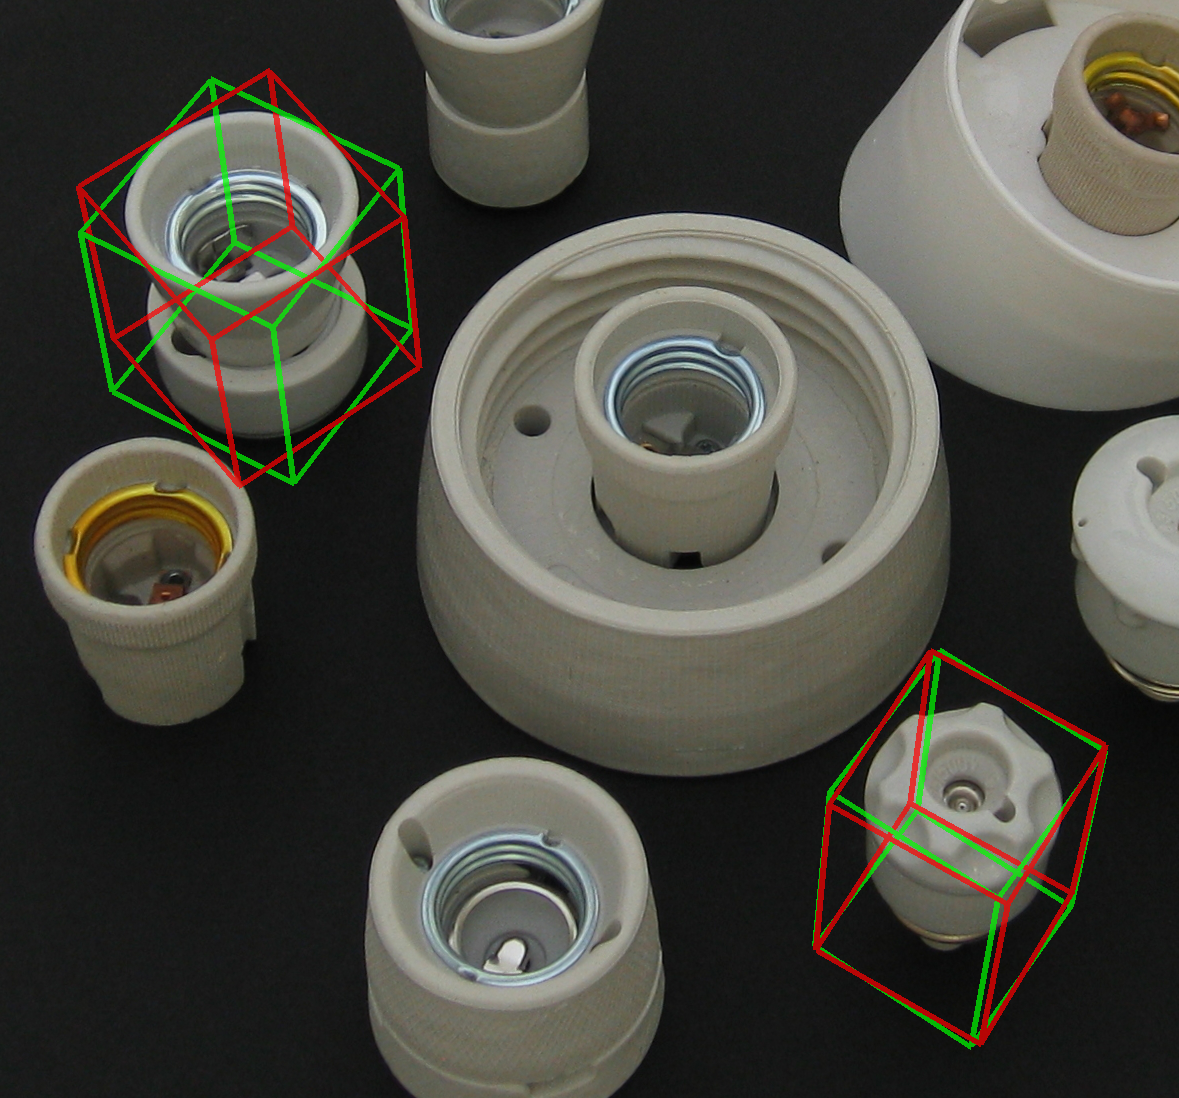
\includegraphics[width=0.8\linewidth]{6dpat_exp_0150}
    	\caption{Image 0150.jpg shows a nearly top-down view.}
    	\label{fig:6dpat_exp_0150}
	\end{subfigure}
	\hfill
	\begin{subfigure}[t]{0.47\textwidth}
	\centering
    	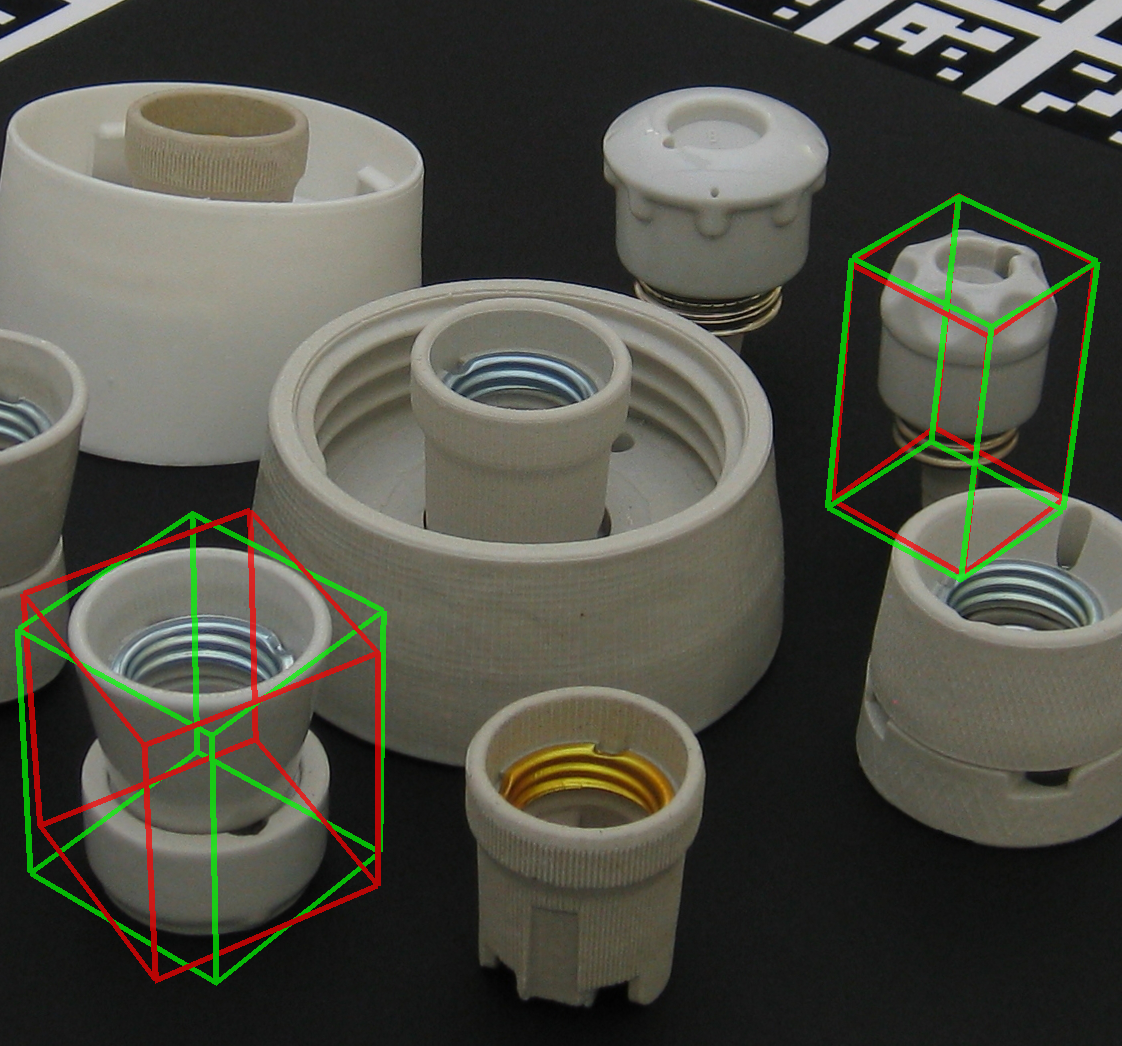
\includegraphics[width=0.8\linewidth]{6dpat_exp_0350}
    	\caption{Image 0350.jpg shows mix of a top-down and sideways view.}
    	\label{fig:6dpat_exp_0500}
	\end{subfigure}
	\caption{Two example frames from test scene 7 of the T-Less dataset annotated using \ac{6dpat}. The green bounding box was derived from the ground-truth pose of the dataset, the red box from our recovered pose.}
	\label{fig:6dpat_exps}
\end{figure} 

The components corresponding to the letters that we use in the following paragraph can be taken from \fig \ref{fig:6dpat_components}. To annotate a new pose, the user has to select an image $I$ from the images gallery, first (see \textit{B} in \fig \ref{fig:6dpat_components}). The pose viewer (see \textit{C} in \fig \ref{fig:6dpat_components}) then displays the image. The object models gallery (see \textit{E} in \fig \ref{fig:6dpat_components}) can be used to select the object model $O$ that the image is to be annoated with. The object model is displayed by the pose editor (see \textit{F} in \fig \ref{fig:6dpat_components}) after selection. The user can rotate the object to view otherwise hidden areas. Using the arrow keys, the user can move the object along the $x$ and $y$ axis and also, by pressing the shift key, along the $z$ axis. 

When the object is in an appropriate position, the user can begin to create a correspondence $C$ by clicking on $I$. This defines the 2D location $u$ of the correspondence on the image. To complete the correspondence, the object model $O$ has to be clicked at the respective 3D point $p$. This procedure has to be repeated until enough correspondences $C_1, \cdots, C_n$ have been defined to recover the new pose $P$. The minimum number of correspondences is $4$. 

The creation process is shown in \fig \ref{fig:6dpat_correspondence_creation}. More correspondences can make the initial pose more accurate. Clicking the \textit{Create} button at the bottom of the pose viewer recovers the pose $P$ by solving the \ac{pnp} problem implied by the correspondences $C_i$ with OpenCV's \textit{solvePnPRansac} method. The newly recovered pose can be refined using the controls of the pose viewer. After pose refinement, it is necessary to click the \textit{Save} button.

Another intuitive way of recovering poses is dragging the object model from the pose editor onto the pose viewer at the approximately correct position. We assumed that the chosen procedure is faster, as clicking correspondences is a swift action which, when executed diligently, can result in immediately accurate poses. It also resembles the way the neural network pipeline recovers poses (see Chapter \ref{chapter:semi_automatic}).

The slider labeled \textit{Transparency} can be used to reduce the object's opacity on the image. After all poses have been annotated successfully, the next image can be selected from the image gallery. This operation has to be repeated until the dataset is fully annotated, although intermediate states can already be used to train the network (see Section \ref{subsection:online_learning}).

It is possible to use the neural network to predict poses. This requires a proper setup and training of the network beforehand. The user can then start the prediction process by clicking the \textit{Predict} button in the lower right corner of the pose editor.

Example times of the manual annotation process (without aid of the network) are given in Table \ref{tabel:6dpat_example_times}. The times in parenthesis show how long it took to click the correspondences, the bold times are the overall time needed. The measured times were achieved by the author of this work trying to recover a single pose of the specified object model. We accepted a pose as correct, when the visual result was subjectively satisfactory. This means that the measurements are not to be seen as an empirical study  but as an indicator of the efficiency of the program. The table shows that the time of clicking correspondences does not linearly scale with the overall length of the annotation process. Recovering the pose for object 01 in image 0250.jpg took less overall time than recovering the pose of object 15 in the same image, but clicking the correspondences took longer.

The quality of the initial pose is crucial for the efficiency, as an accurate initial pose needs less corrections. \fig \ref{fig:6dpat_exps} shows two of the example images used for annotation. One of the reasons why the times of recovering poses vary significantly is the angle between the camera and the object. The nearly top-down view in image 0150.jpg prevents clicking correspondences along the object's $z$-axis, which is the largest dimension of the object. The mix of the top-down and sideways view in image 0350.jpg allows to click many correspondences along all axes which makes the initial pose more accurate. 

The rotational discrepancy of the object on the left in the two images is a result of missing characteristics of the 3D model which are part of the real-world counterpart. This made it difficult to recover the pose properly. We neglected this error because the rotation is offset by a similar amount in all annotated images (see Appendix \ref{appendix:example_annotations}). The object model on the right has a notch at the top which prevents this rotation error. This issue is discussed further in the next section.

\begin{figure}[!tbp]
	\centering
    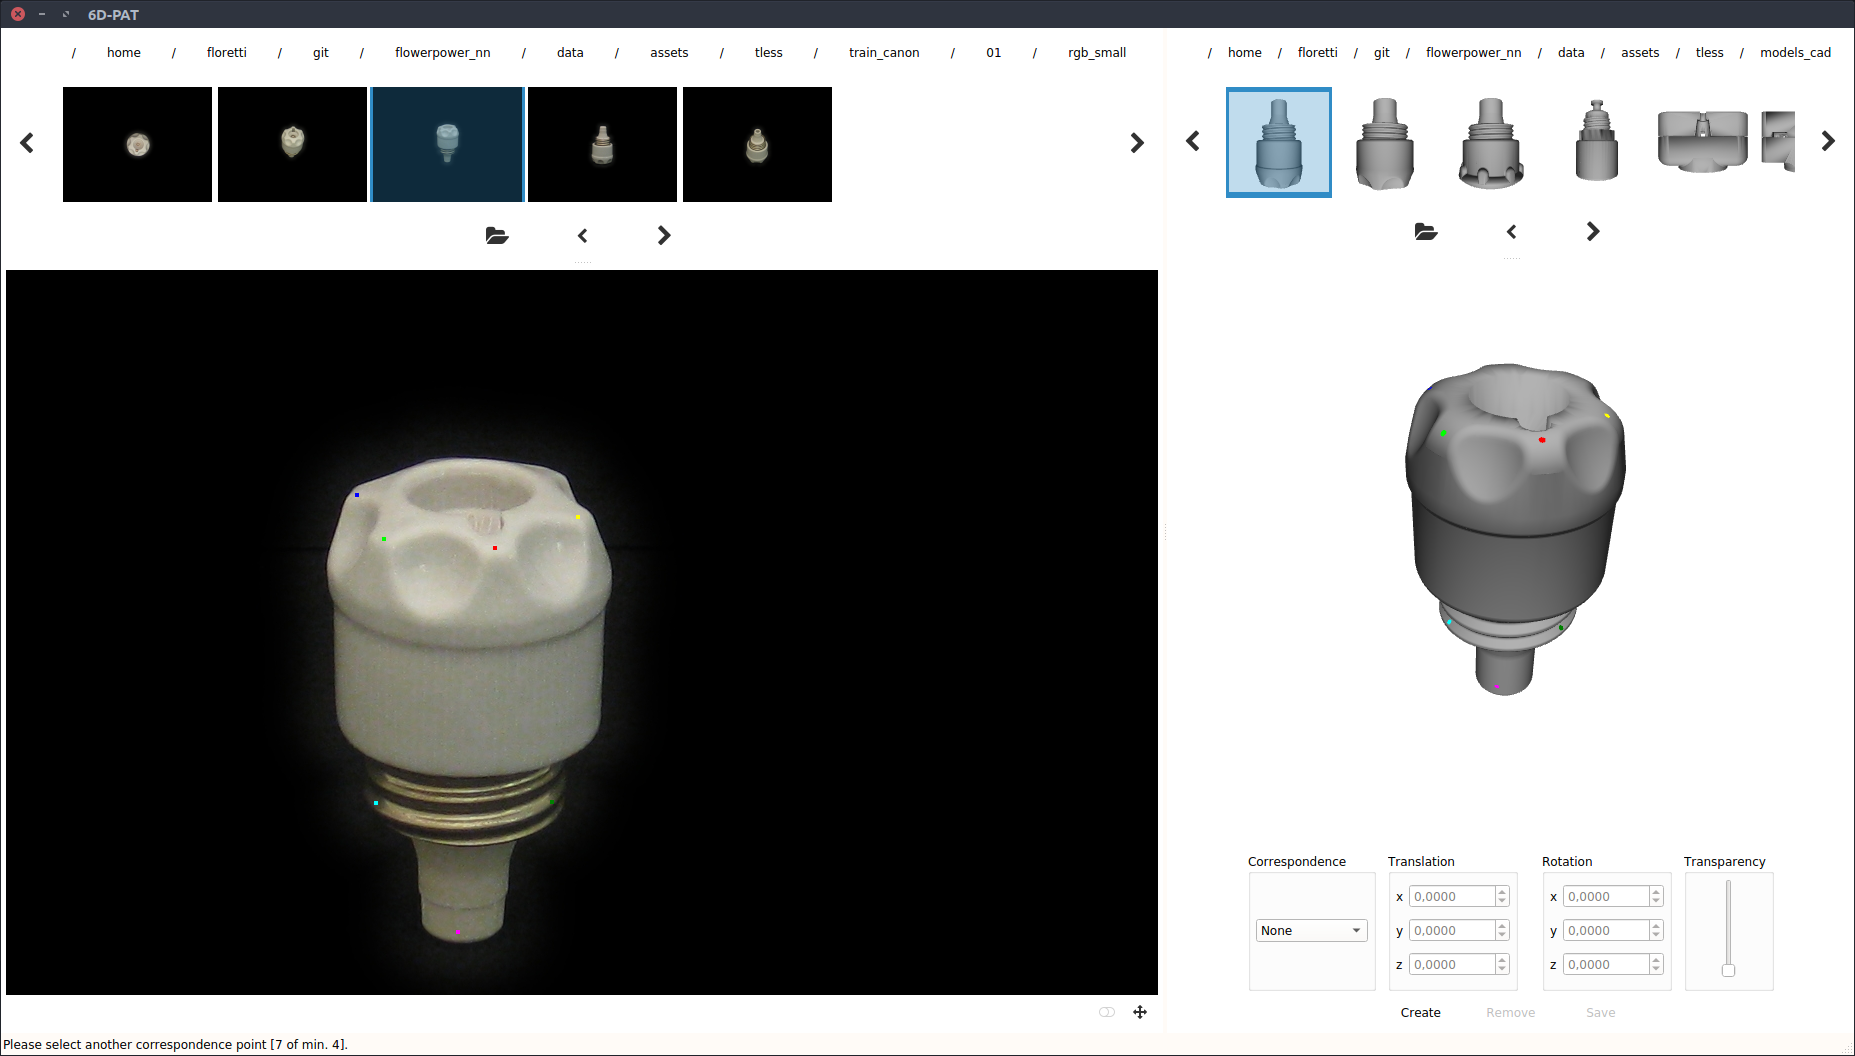
\includegraphics[width=\linewidth]{6dpat_correspondence_creation}
    \caption{The pose creation process. The user has to click the image first and then the corresponding 3D location on the object model. The red circles and red lines were added afterwards to emphasize the colored dots drawn by the program.}
    \label{fig:6dpat_correspondence_creation}
\end{figure} 

\subsection{Problems \& Difficulties} \label{section:6dpat_difficulties}

During the implementation of the program, multiple problems arose and complicated the development process. We summarize the most important ones and explain issues which impacted the final design.

One of the major factors that prolonged the implementation process was that we used \textit{Qt3D} to realize all graphical processing at first. Qt3D is part of the main Qt framework. Qt3D's purpose is to encapsulate graphics programming to increase portability of applications including 3D graphics. The incomplete documentation and unintuitive concepts make it difficult to use without consultation. After complications still emerged in the almost completed annotation tool, the Qt3D framework was deemed unusable and omitted in favor of a native OpenGL implementation.

Initially, a desired feature was to present another unannotated image after the user finishes annotating all poses in the current image. This is not feasible for multiple reasons. First of all, a user might still not be content with the poses. Selecting the next image programmatically could happen too early and thereby disrupt the annotation process of the user. The datasets can also have very distinct characteristics, which require the user to choose the next image manually. For a dataset like T-Less, many images have to be skipped due to their similarity. A network trained on one view on an object only, will likely predict inaccurate poses for a different view showing other characteristics of that object. The dataset of the Endoscopic Vision Challenge has less similar consecutive images.

The diversity of available datasets (see Chapter \ref{chapter:experiments} for a selection of datasets) is also the reason why the program does not provide functionality to initialize the next poses based on the ones in the last image. This feature would imply too many assumptions on the dataset and, in the worst case, cause more work for the user. 

While trying to annotate the images of the Endoscopic Vision Challenge dataset, it became clear that proper 3D models are crucial for successful annotation. To temporarily annotate the medical images, 3D surgical tools were downloaded from the internet as a replacement for the missing object models. But having a different shape and also missing the distinctive features of the real objects makes it very difficult to estimate the ground-truth pose. The influence of contradicting annotated poses during training of a network is not clear. The author of this work strongly recommends to obtain the correct 3D models before annotating the Endoscopic Vision Challenge images. The issue of the object models not fitting the segmentation mask can be seen in \fig \ref{fig:sfb_segmentation}. \fig \ref{fig:sfb_original} shows the actual image and the discrepancy between the object models and image pixels.

\begin{figure}
	\begin{subfigure}[t]{0.47\textwidth}
		\centering
    	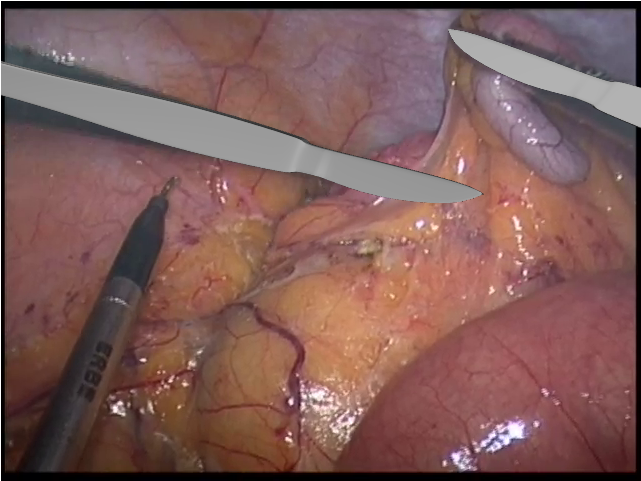
\includegraphics[width=\linewidth]{6dpat_sfb_image}
    	\caption{An image from the medical images dataset annotated using \ac{6dpat}. The correct rotation and translation are difficult to estimate without the correct 3D models.}
    	\label{fig:6dpat_sfb_image}
	\end{subfigure} 
	\hfill
	\begin{subfigure}[t]{0.47\textwidth}
		\centering
    	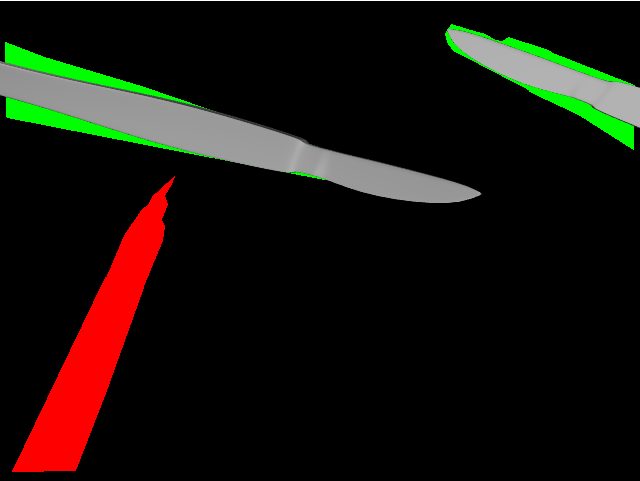
\includegraphics[width=\linewidth]{6dpat_sfb_segmentation}
    	\caption{The corresponding segmentation image. The discrepancy between the segmentation masks and the object model is the clearly visible green area.}
    	\label{fig:6dpat_sfb_segmentation}
	\end{subfigure} 
	\caption{Example annotations of images of the Endoscopic Vision Challenge dataset. The object model is taken from \cite{3d_scalpel_online}.}
	\label{fig:6dpat_sfb}
\end{figure} 

A general problem of any dataset can be seen in Appendix \ref{appendix:example_annotations} in form of the rotational error of manually annotated images. If the offset is similar in all recovered poses, this might not cause any trouble. If not, a network might be trained with contradicting object coordinates. There is no simple solution to this problem. Distinct characteristic of the object models could reduce this effect significantly, like the letters on the surgical tools in the Endoscopic Vision Challenge dataset or the notch of object model 01 of the T-Less dataset.

A first try to use the official Python bindings did not work to our complete satisfaction. Including the bindings in the program required complex alterations. Running Python scripts is also possible by starting a new process. Qt natively offers this functionality. Starting a new process was thus favored over including Python directly in the C++ code.

The Python binding is not complete, yet. Training is not possible and a deep learning expert has to setup the network and its parameters to enable its usage in the program. The current state of the incorporation of the network is to be seen as a proof of concept that requires further development.

Because the neural network is trained for one object only, the time-intensive step (proportional to the overall time needed for inference on one image) of loading the trained weights has to be performed before predicting poses for different objects. The frame of this work was to explore neural networks trained for one object only, it is therefore not known whether this overhead of loading the weights can be reduced.

\subsection{Future Improvements}

To provide an outlook how the program can be improved in the future, we mention solutions to some of the problems of Section \ref{section:6dpat_difficulties}. An important feature that should be implemented is allowing to move the object models around on the displayed image by dragging and rotating them using the mouse. The initial poses using the clicking procedure are already sufficiently accurate in many cases. But when the camera is looking along an axis of the object, the rotation can be far off. The user can correct these poses with the provided controls. The described editing process could profit from this functionality in terms of time needed per annotation. To provide the user with a better overview of the image and its annotated poses, a zoom option should be implemented, as well.

The binding of the neural network to the program does not allow to load the weights of the net and persist this state in the memory of the computer. In case that the user wants to annotate a large dataset of just one object, they could profit from a feature allowing to keep the weights in memory instead of loading them each time the inference process is started. This way, predicting the pose for only one image could be achieved in significantly less time. Running the network to predict the pose of one object in a large amount of images amortizes the loading of the weights.

Another suggested step is to fully incorporate the network in the annotation tool. This way, inexperienced users can profit from the network without the need for an expert to run the network inference. There is probably no way to automatize the setup process, as this requires knowledge neural networks. In an ideal setting, this interference can be reduced to a minimum and users are introduced to the most relevant parameters only, which they can set from within the program.